\sloppy

Les ambitions de la mission Défense et Sécurité sont aujourd’hui implémentées à travers un centre d’excellence dédié au domaine de la Sécurité et Défense afin de faciliter le développement et le transfert à court, moyen et long terme de technologies issues de la Recherche.

Ce chapitre est celui dans lequel nous allons présenter les projets sur les quels nous avons travailler, notre méthodologie de travail, leur analyse et les résultats obtenus durant notre alternance au seins de l'Inria.

\section{Projet IntelLab : Application Web}

\subsection{Contexte du projet}

IntelLab est un environnement de \textbf{simulation, formation, et d’expérimentation}. Il vise d’une part à faire appréhender aux académiques et aux entreprises les problèmes concrets rencontrés par les opérationnels afin d’y proposer des solutions communes, et d’autre part, de permettre d’expérimenter les solutions sur la base de procédures de tests opérationnels.

\noindent Les plateformes du projet IntelLab permettent de jouer deux types de scénarios :

\begin{itemize}\addtolength{\itemsep}{-0.35\baselineskip}%
	\item Des scénarios simulant l'exploitation du renseignement d'intérêt militaire ;
	\item Des scénarios de type sécurité économique (détection de signaux faibles précurseurs d'actions d'ingérence).
\end{itemize}

\subsection{Moyens mis à la disposition des équipes de développement}
Dans le cadre de ce projet, l'équipe de développement est composée uniquement du responsable informatique et de moi-même. Cela signifie que nous avons adopté une approche \textit{agile et collaborative} pour gérer le projet.


\subsection{Outils de gestion de projet}

Les projets sont suivis lors de réunions hebdomadaires et de séminaires semestriels, où chaque membre de l'équipe évalue les progrès, identifie les problèmes et propose des corrections pour atteindre les objectifs fixés.
En complément, des échanges bilatéraux hebdomadaires entre responsables et membres de l'équipe permettent de prendre des décisions plus rapidement et efficacement, en se concentrant sur des discussions plus ciblées que lors des réunions d'équipe générales.

\subsubsection{Définition des objectifs et des exigences du projet}

Il était important de recueillir les exigences et attentes de l’application.
Grâce à cela nous avons planifié notre travail en fonction des priorités et urgences. Cette planification a été faites sur GitLab sous forme d’issues différenciés par des labels (backend, frontend, bug, …).
Ces labels nous permettent de déterminer dans quoi et ou à quelle partie correspondes les issues.

\subsubsection{Planification des tâches}

Pour le projet IntelLab, notre méthode de travail est fortement axée vers la méthodologie agile car les priorités du développement varient régulièrement en fonction du calendrier des scénarios joués ou à jouer sur les applications.
Le responsable informatique Jonas Renault étant chargé de la planification, a choisi d'utiliser la plateforme de gestion de code source GitLab.

\begin{figure}[h]
	\center
	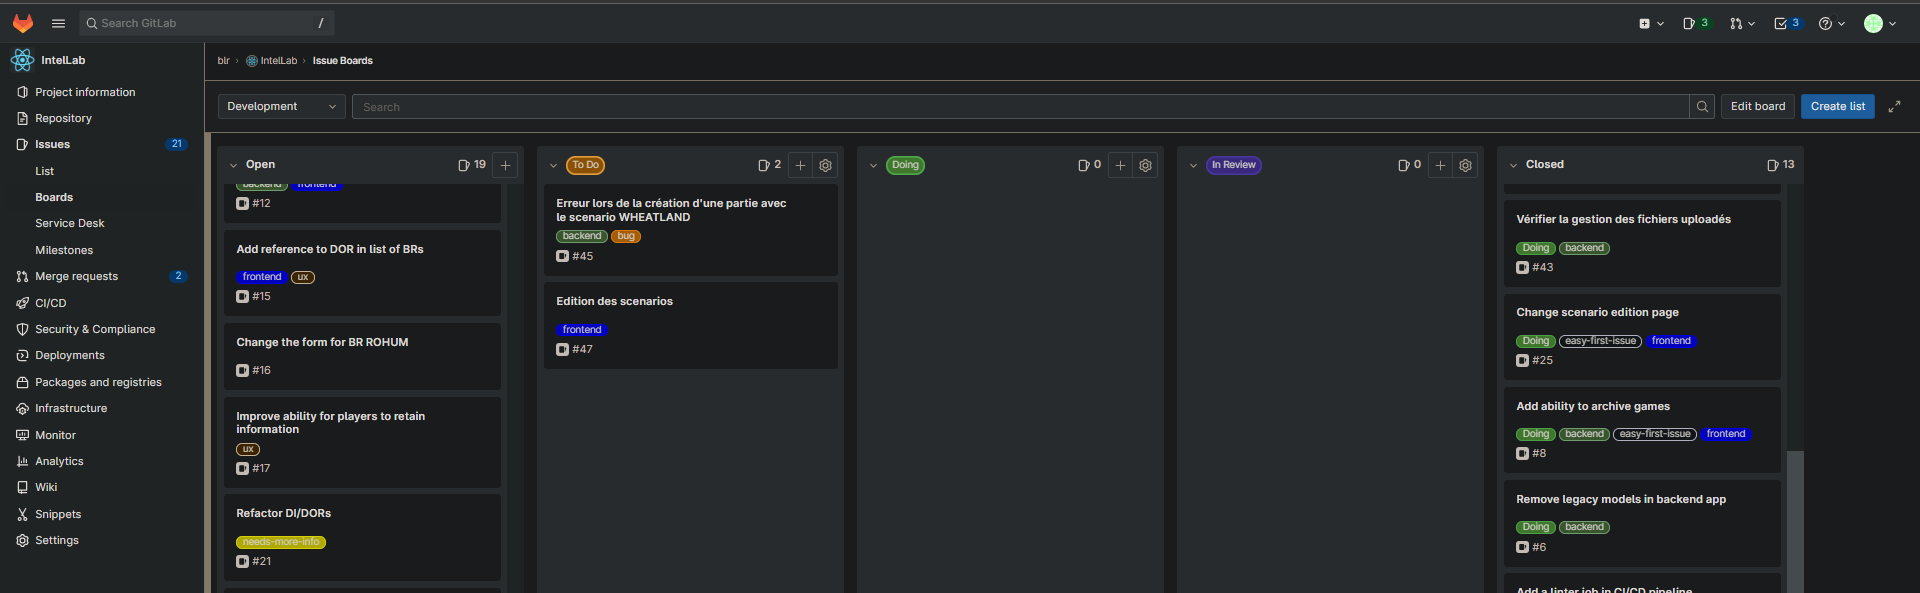
\includegraphics[width=\textwidth]{./images/gitlab_intellab.PNG}
	\caption[Planification des issues]{Planning issues - GitLab}\label{fig:gitlab_intellab}
\end{figure}

GitLab est une plateforme de gestion de code source basée sur Git qui permet aux équipes de développeurs de collaborer sur des projets de logiciels, de suivre les modifications du code source et de gérer des versions de code.
Elle offre des fonctionnalités pour la collaboration en temps réel, l'intégration continue et la livraison continue, la gestion de projet.


\subsection{Réalisation du projet}
IntelLab anciennement appelé \textbf{BLR (Battle Lab Rens)} a été initialement développé par un ancien ingénieur. Le BLR avait pour objectif la simulation exclusive des scénarios des services de renseignements militaires.
Dans l’optique de rendre l’application plus générique afin qu’elle s’adapte à d’autres types de scénarios autres que le renseignement militaire, le responsable informatique et moi avions procédé à la refonte complète de l’application en commençant par le changement de nom.


\subsubsection{Analyse du code existant et développement de la plateforme}

Avant de commencer le développement de l’application, nous avons effectué une analyse approfondie du code et de l’infrastructure du projet.
Ce qui nous a permis de mettre en place une logique de travail sur la restructuration de tout le projet.

Nous avons fait une refonte complète de l’application. La refonte avait pour but de restructurer le code afin de pouvoir poursuivre le développement de fonctionnalités nouvelles et de nouvelles fonctionnalités.
En parallèle, nous avons rédigé des tests unitaires et fonctionnelle pour garantir l'absence de détérioration dans la logique fonctionnelle de l'application après avoir effectué le remaniement du code que nous avons orchestré.


\subsubsection{Infrastructure des serveurs de développement et de production}

Il n'existait pas de serveur de développement sur lequel nous pouvions effectuer des tests de déploiement. Nous avons mis en place un serveur de développement qui sera par la suite la réplique parfaite du serveur de production.
Nous avons choisi d'utiliser Docker comme environnement d'exécution, installé sur un système d'exploitation Ubuntu Server.
La conteneurisation de nos serveurs nous offre une grande flexibilité dans la gestion des composants de notre application.
Ce serveur sert à vérifier le bon fonctionnement de l'application avant sa mise en production.

Les serveurs du backend, du frontend, du broker MQTT et de la base de données sont automatiquement installés dans l'environnement Docker des serveurs de développement et de production.
Cela est possible grâce au déploiement continu depuis GitLab que nous avons configuré, ce qui nous fait gagner énormément de temps pendant le déploiement.


\subsubsection{Description de l'infrastructure logicielle}

Cet environnement est développé en utilisant les technologies suivantes :

\begin{itemize}
	\item \textbf{Frontend} : ReactJS, gère l’interface utilisateur ;
	\item \textbf{Backend} :
	      \begin{itemize}
		      \item \textit{NodeJS} et \textit{ExpressJS} pour la partie serveur web ;
		      \item \textit{PostgreSQL} est le système de gestion de base de données ;
		      \item \textit{Sequelize} est utilisé pour les requêtes entre le serveur et la base de données ;
		      \item \textit{MQTT} : Il fournit une méthode de communication asynchrone de messages entre deux ou plusieurs appareils connectés à un réseau.
	      \end{itemize}
	\item \textbf{Infrastructure} :
	      \begin{itemize}
		      \item \textit{Docker} : Utilisé pour le déploiement de l’application sur les serveurs de test et de production ;
		      \item \textit{GitLab} : notre projet y est répertorié pour le travail collaboratif, les tests unitaires, les tests d’intégration, déploiement et intégration automatique.
	      \end{itemize}
	\item \textbf{Tests} :
	      \begin{itemize}
		      \item \textit{Vitest} : Outils de gestion des tests côté frontend ;
		      \item \textit{Jest} : Outils de gestion des tests côté backend.
	      \end{itemize}
\end{itemize}


\begin{figure}[h]
	\center%
	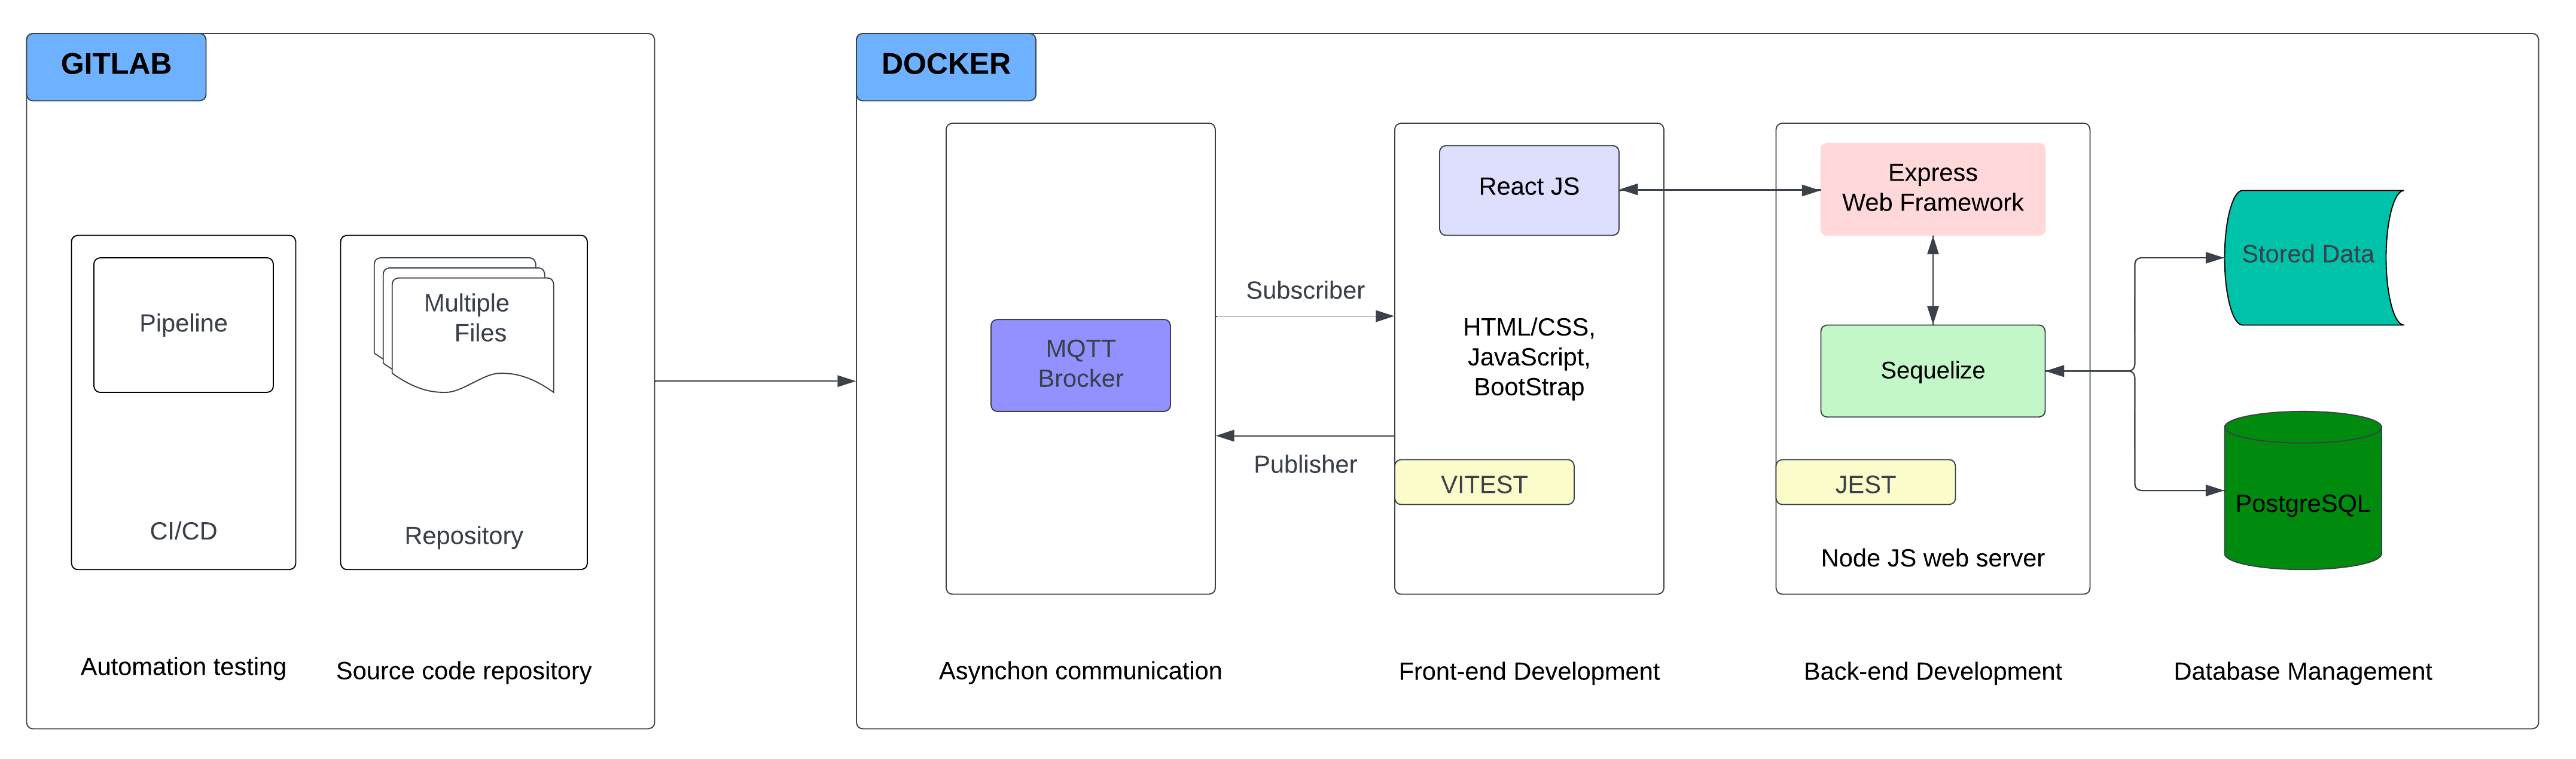
\includegraphics[width=\textwidth]{./images/architectur_intellab.png}
	\caption[Architecture Application Web IntelLab]{Architecture Application Web IntelLab}\label{fig:architectur_intellab}
\end{figure}


\subsection{Stratégie de tests}

En tant qu'environnement de simulation, formation et expérimentation, la fiabilité et la qualité d’IntelLab sont d'une importance capitale pour atteindre les objectifs visés par cette plateforme.
IntelLab est une application de recherche, donc nous n’avons pas les mêmes attentes ni besoins en termes de stratégie de tests.


\subsubsection{Objectifs et critères de tests}
Les tests sur IntelLab visent à assurer que l'application répond aux exigences fonctionnelles, en permettant des simulations réalistes et fiables des scénarios de renseignement.
Ils visent également à garantir la stabilité et la sécurité des données, à détecter et corriger les anomalies pendant les exercices, et à améliorer l'ergonomie et la convivialité de l'application pour une meilleure expérience utilisateur.


\subsubsection{Mise en place des outils de tests}

\begin{itemize}\addtolength{\itemsep}{-0.35\baselineskip}%
	\item \textbf{Outils de gestion des tests }: Nous utilisons l'outil de gestion des tests \textbf{vitest} coté frontend et \textbf{jest} coté backend pour suivre nos cas de test, les résultats des tests et les anomalies détectées.
	      \begin{figure}[h]
		      \center
		      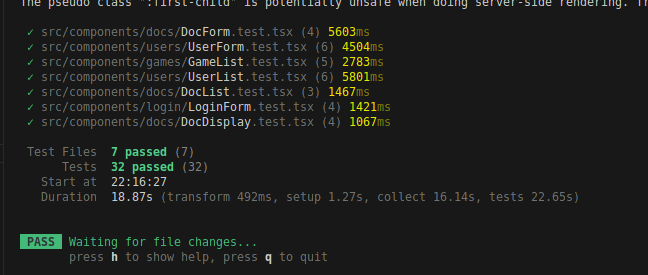
\includegraphics[scale=0.7]{./images/test_frontend_il.png}
		      \caption[Rapport test frontend avec VITEST]{Rapport tests avec VITEST}\label{fig:test_frontend_il}
	      \end{figure}
	\item \textbf{Outils d'automatisation des test} : Nous utilisons les pipelines de GitLab pour automatiser l'exécution des tests.
	      \begin{figure}[h]
		      \center
		      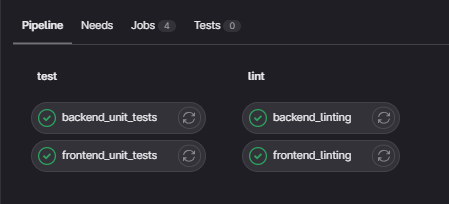
\includegraphics[scale=0.9]{./images/pipeline_tests.png}
		      \caption[pipeline des tests automatiques]{pipeline des tests automatiques}\label{fig:pipeline_tests}
	      \end{figure}
\end{itemize}


\subsubsection{Rédaction des procédures de tests}

\begin{itemize}
	\item \textbf{Scénarios de test} : Chaque scénario est accompagné de données de test spécifiques et de critères de succès clairement définis.
	\item \textbf{Procédures de test} : Nous documentons les procédures de test pour chaque type de test afin de garantir une exécution cohérente.
	\item \textbf{Critères d'acceptation} : Nous établissons des critères d'acceptation clairs pour chaque scénario de test, définissant ce qui est considéré comme un test réussi.
\end{itemize}

\begin{table}[h]
	\centering
	\begin{tabular}{|p{1.1cm}|p{3cm}|p{3cm}|p{4cm}|p{3cm}|}
		\hline
		\textbf{Menu Name} & \textbf{Description}                & \textbf{Test data}                & \textbf{Expected Output}                                     & \textbf{Actual Output}                                       \\ \hline
		Login              & should render a sign in button      & -                                 & Se connecter                                                 & Se connecter                                                 \\ \hline
		Login              & should display required helper text & Username: empty Password: Empty   & Le nom d'utilisateur est requis. Un mot de passe est requis. & Le nom d'utilisateur est requis. Un mot de passe est requis. \\ \hline
		Login              & should login user                   & Username: john Password: johnjohn & Connexion réussie                                            & Connexion réussie                                            \\ \hline
		Login              & should handle server errors         & Username: john Password: johnpass & Incorrect email or password                                  & Incorrect email or password                                  \\ \hline
	\end{tabular}
	\caption{Scénarios de test}
	\label{tab:test_scenarios}
\end{table}


\section{Projet IntelLab : Serveur de messagerie}

Ce projet a beaucoup de similitudes que celui de l'application Web. Nous allons ressortir quelques paries avec leur différences :


\subsection{Contexte du projet}
Le contexte initial de ce projet est pratiquement le même que celui de l'application web, la différence réside au niveau du type de scénario.
Ce projet permet la simulation des scénarios de types sécurité économique.
Ce type de scénario a exigé le développement d'un autre d'environnement car diffère du monde du renseignement militaire.
Cette plateforme est née du fait qu'on doit recréer un environnement d’entreprise telles que des startups ou des équipes de recherche.
Les objectifs la formation et la sensibilisation à la détection de signaux faibles précurseurs d’actions d’ingérence.


\subsection{Outils de gestion de projet}
Comme pour les autres projets, nous sommes une équipe de deux personnes, le responsable informatique et moi. Au vu de cela, nous avons toujours adopté la méthodologie agile car cela nous permet de gérer efficacement nos ressources limitées, de nous adapter rapidement aux changements de priorités, et de livrer des fonctionnalités clés du serveur de messagerie de manière itérative et continue, en garantissant une meilleure réactivité aux besoins des utilisateurs finaux.

\subsubsection{Planification des tâches}
Comme pour l'autre projet, nous avons centralisé la gestion de ce projet sur la plateforme GitLab.
La description des taches, la gestion du code, collaboration en temps réel, l’intégration continue et le déploiement automatique, toutes ses fonctionnalités sont gérées sur la plateforme GitLab.

\begin{figure}[h]
	\center
	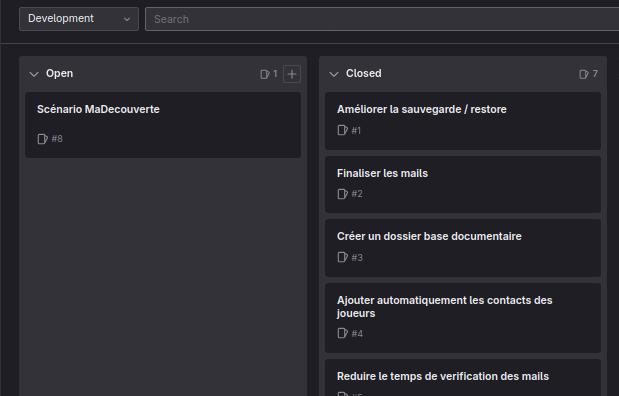
\includegraphics[width=0.6\textwidth]{./images/gitlab_mpc.png}
	\caption[Planification des issues MPC]{Planning issues MPC - GitLab}\label{fig:gitlab_mpc}
\end{figure}


\subsection{Réalisation du projet}

\subsubsection{Etude de l'existant}

Dans le cadre du projet de serveur de messagerie, nous avons étudié l'infrastructure existante.
Cette infrastructure présente un serveur de messagerie utilisant \textit{HmailServer}, avec \textit{Mozilla Thunderbird} et \textit{Outlook} pour les utilisateurs finaux.

L'ancienne infrastructure reposait sur l'installation d'HmailServer sur un PC dédié en local, non utilisé par les joueurs, et nécessitait la configuration de répéteurs WiFi pour permettre la connectivité des utilisateurs au réseau de messagerie.
Les adresses IP et les noms de domaine devaient être manuellement configurés pour garantir la connexion des PC clients au PC contenant le serveur de messagerie.
La gestion des comptes de messagerie était effectuée via HmailServer, où chaque domaine et adresse étaient créés manuellement avant d'être ajoutés dans Mozilla Thunderbird et ou Outlook.

Cette approche offrait une solution locale robuste, mais nécessitait une configuration minutieuse et fastidieuse, notamment lors de changements d'adresses IP ou de la configuration des serveurs SMTP dans Thunderbird.
Nous avons également souligner des limitations, telles que la nécessité d'ouvrir certains ports spécifiques pour que le serveur puisse fonctionner correctement sur certains PC, ce qui impliquait l'intervention de la DSI.

L'étude de cette infrastructure existante a permis d'identifier les points forts et les limites de l'ancien système, ce qui nous guidera dans l'optimisation et la modernisation du nouveau projet de serveur de messagerie.


\subsubsection{Nouvelle infrastructure du serveur de messagerie}



Le projet de serveur de messagerie utilise une infrastructure basée sur Docker pour les environnements de développement et de production. Docker permet de containeriser les différents services nécessaires au fonctionnement du serveur de messagerie, offrant ainsi une grande flexibilité et une gestion simplifiée des déploiements. Cette approche permet également de maintenir des environnements cohérents entre le développement et la production, assurant une transition fluide et sans heurts.

Les services critiques, tels que le serveur SMTP, IMAP, l'interface d'administration, ainsi que les services auxiliaires comme le résolveur DNS, sont déployés dans des conteneurs Docker distincts. Cette architecture modulaire permet une maintenance facilitée et un déploiement rapide des mises à jour.

\subsubsection{Description de l'infrastructure}

Cet environnement est développé en utilisant les technologies et outils suivants :

\noindent\textbf{Core services :}
\begin{itemize}
	\item \textbf{Mailu :} Nn serveur de messagerie simple mais complet, facile à configurer et facile à entretenir et complet, sous forme d'un ensemble d'images Docker. Les principales caractéristiques comprennent :
	      Un ensemble d'images Docker utilisées pour configurer et gérer le serveur de messagerie. Les services principaux incluent :
	      \begin{itemize}
		      \item \textbf{Serveur de messagerie standard,} IMAP et IMAP+, SMTP et soumission avec profils de configuration automatique pour les clients.
		      \item \textbf{Fonctionnalités de messagerie avancées,} alias, alias de domaine, routage personnalisé, recherche en texte intégral des pièces jointes des e-mails
		      \item \textbf{Accès Web (Roundcube),} Fournit les services IMAP pour l'accès aux boîtes aux lettres.
		      \item \textbf{Fonctionnalités utilisateur,} alias, réponse automatique, transfert automatique, comptes récupérés, managesieve.
		      \item \textbf{Fonctionnalités d'administration,} Un service de filtrage de spam qui analyse et marque les emails suspects.
		      \item \textbf{Sécurité,} TLS appliqué, DANE, MTA-STS, Letsencrypt!, DKIM sortant, scanner antivirus, Snuffleupagus , blocage des pièces jointes malveillantes.
		      \item \textbf{Antispam,} uto-apprentissage, liste grise, DMARC et SPF, anti-usurpation d'identité.
		      \item \textbf{Liberté,} tous les composants FOSS, aucun tracker inclus.
	      \end{itemize}
\end{itemize}

\begin{figure}[h]
	\center
	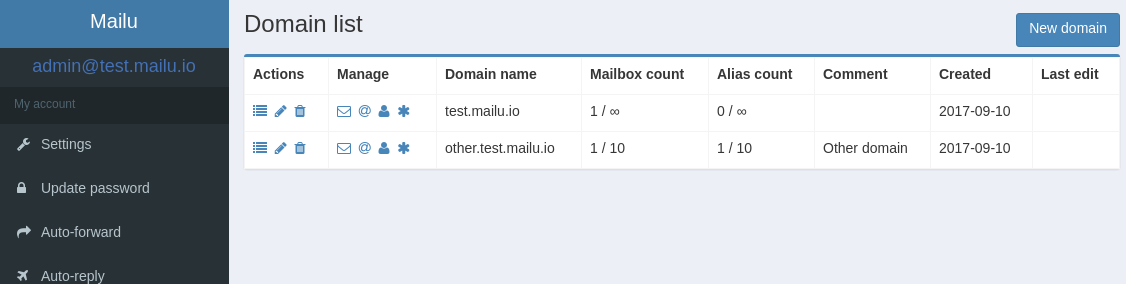
\includegraphics[width=\textwidth]{./images/domains_mailu.png}
	\caption[Domaines du serveur Mailu]{Liste des domaines sur le serveur Mailu}\label{fig:domains_mailu}
\end{figure}

\noindent\textbf{Scripts d'administration :}
\begin{itemize}
	\item \textbf{setup-users :} Script pour configurer les comptes utilisateurs sur le serveur de messagerie.
	\item \textbf{setup-emails :} Script pour initialiser les boîtes aux lettres des utilisateurs avec les messages préconfigurés.
	\item \textbf{backup.sh :} Script utilisé pour sauvegarder les mails des joueurs d'une session de jeu.
	\item \textbf{reset.sh :} Script utilisé pour réinitialiser et reconfigurer le serveur de messagerie.
	\item \textbf{restore.sh :} Script utilisé pour restaurer les mails d'une session antérieure pour des fins statistiques et amélioration des scénarios.
\end{itemize}

\noindent\textbf{Infrastructure :}
\begin{itemize}
	\item \textbf{Docker :} Utilisé pour déployer et orchestrer l'ensemble des services de messagerie sur les serveurs de développement et de production.
	\item \textbf{Poetry :} Utilisé pour gérer les dépendances Python et les scripts d'administration du serveur.
\end{itemize}

\begin{figure}[h]
	\center
	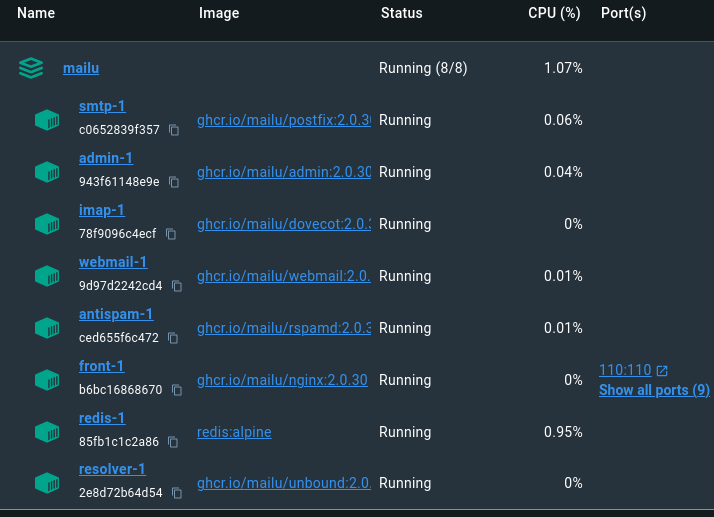
\includegraphics[width=0.6\textwidth]{./images/docker_mpc.png}
	\caption[Liste des conteneurs de Mailu]{Containers Mailu}\label{fig:docker_mpc}
\end{figure}


\subsubsection{Avantages de la nouvelle infrastructure}

La nouvelle infrastructure présente plusieurs avantages par rapport à l'ancienne :

\begin{itemize}
	\item \textbf{Flexibilité et Scalabilité :} L'utilisation de Docker pour containeriser les différents services permet une grande flexibilité dans la gestion des composants du système. Cette approche facilite le déploiement, la mise à jour, et la maintenance des services, tout en permettant de faire évoluer l'infrastructure selon les besoins croissants sans perturber les opérations en cours.
	\item \textbf{Automatisation et Gestion Simplifiée :} L'intégration de scripts d'administration pour la configuration des comptes utilisateurs, initialisation des boîtes mails, la sauvegarde, la réinitialisation et la restauration des données simplifie considérablement la gestion du serveur de messagerie. Ces scripts automatisent des tâches qui, auparavant, auraient pu nécessiter une intervention manuelle complexe et fastidieuse, réduisant ainsi les risques d'erreur humaine et améliorant l'efficacité opérationnelle.
\end{itemize}




% --------------------------------------------------------------------------
\section{Projet Détection et reconnaissance de véhicules militaires sur des images et vidéos (DetReco)}

\subsection{Context du projet DetReco}

Cette mission s’inscrit dans le cadre d’une collaboration entre l’équipe STARS du centre de Sophia-Antipolis, la Direction Générale de l’Armement (DGA) et le département Défense et Sécurité de l’Inria.

L'objectif de ce projet consiste à mener une étude de l’état de l’art des algorithmes pouvant s’appliquer à la détection et à la reconnaissance, proche du temps réel, de véhicules militaires sur des images et vidéos; de proposer une implémentation de cet état de l’art fusionnant éventuellement plusieurs approches; ainsi que d’en faire une évaluation.
L’évaluation consistera non seulement en une quantification globale des performances mais aussi une mesure plus fine des erreurs de traitement (faux positifs, silence).


\subsection{Méthodologie}
La méthodologie du projet DetReco repose sur plusieurs étapes clés :
\begin{enumerate}
	\item \textbf{Préparation des données :} Extraction et annotation d'images provenant de bases de données existantes. telles qu'ImageNet, OpenImages et Roboflow, complétées par des images collectées via des outils de scraping.
	\item \textbf{Entraînement du modèle :} Utilisation de ces données pour affiner un modèle.
	\item \textbf{Suivi des objets :} Application du modèle entraîné pour suivre les véhicules militaires dans des séquences vidéo.
	\item \textbf{Génération d'images :} Utilisation de techniques pour créer des images supplémentaires de véhicules militaires sous diverses conditions.
\end{enumerate}

\subsubsection{Définition des classes}

Afin de développer un modèle capable de faire la différence entre différents types de véhicules militaires, nous allons définir des classes larges en utilisant la catégorie \textit{Véhicules militaires par type} de Wikipédia.

Nous utiliserons 4 classes :

\begin{itemize}
	\item \textbf{Véhicule de combat blindé (AFV) :} Il s'agit d'un véhicule de combat protégé par un blindage, combinant généralement mobilité opérationnelle avec des capacités offensives et défensives. Les AFV peuvent être à roues ou à chenilles. Des exemples d'AFV incluent les chars(tanks), les véhicules blindés de combat, les canons d'assaut, les canons automoteurs, les véhicules de combat d'infanterie (IFV) et les transporteurs blindés de troupes (APC).
	\item \textbf{Transport de troupes blindé (APC) :} C'est un type de véhicule militaire blindé conçu pour transporter du personnel et du matériel en zone de combat.
	\item \textbf{Véhicule du génie militaire (MEV) :} Ce véhicule est conçu pour les travaux de construction ou pour le transport des ingénieurs de combat sur le champ de bataille.
	\item \textbf{Véhicule blindé léger (LAV) :} Il s'agit de la catégorie de véhicules militaires la plus légère. Un véhicule à quatre roues motrices de type Jeep, destiné à un usage militaire, avec un blindage léger ou sans blindage. \textit{Véhicule de reconnaissance (RV)} est un véhicule militaire utilisé pour des missions de reconnaissance avancée. Les véhicules de reconnaissance à roues et à chenilles sont en service.
\end{itemize}

\subsubsection{Préparation des données}

\indent \textbf{Prepare-01 :} Nous commençons par créer un ensemble de données d'entraînement à partir d'images disponibles dans des ensembles de données de détection (dataset) d'objets open source. (ImageNet, OpenImages, Roboflow).

\begin{itemize}
	\item \textbf{ImageNet : }Le premier dataset que nous avons utilisé est ImageNet21k. De ce dataset, nous avons pu avoir 378 images annotées de tanks.
	\item \textbf{OpenImages : } Dans ce dataset, nous avons réussi à charger 1246 images annotées de tanks.
	\item \textbf{Roboflow : } Nous disposons désormais de 1624 images annotées de tank, mais cela reste insuffisant pour un entraînement optimal du modèle. Pour obtenir encore plus d'images d'entraînement, nous avons charger un autre dataset annotées de véhicules militaires, mis à disposition par \textit{Tuomo Hiippala du Digital Geography Lab}.
\end{itemize}

\noindent Pour cette première étape, nous avons réussi à collecter \textbf{2666 images} de tanks dont \textbf{89 images} non annotées.\\


\noindent\textbf{Prepare-02 :} Nous utilisons également des outils de scraping pour collecter davantage d'images de véhicules militaires à partir d'images Google.

\noindent Nous avons collectés 669 images de plus, ce qui nous fait un total de \textbf{3335 images}.

Ce nombre d'images nous permet de définir quatre grandes classes de véhicules militaires que notre modèle peut ensuite discriminer : \textbf{Armoured Fighting Vehicle (AFV), Armoured Personnel Carrier (APC), Military Engineering Vehicle (MEV) and Light Armoured Vehicle (LAV)}.


\begin{figure}[h]
	\center
	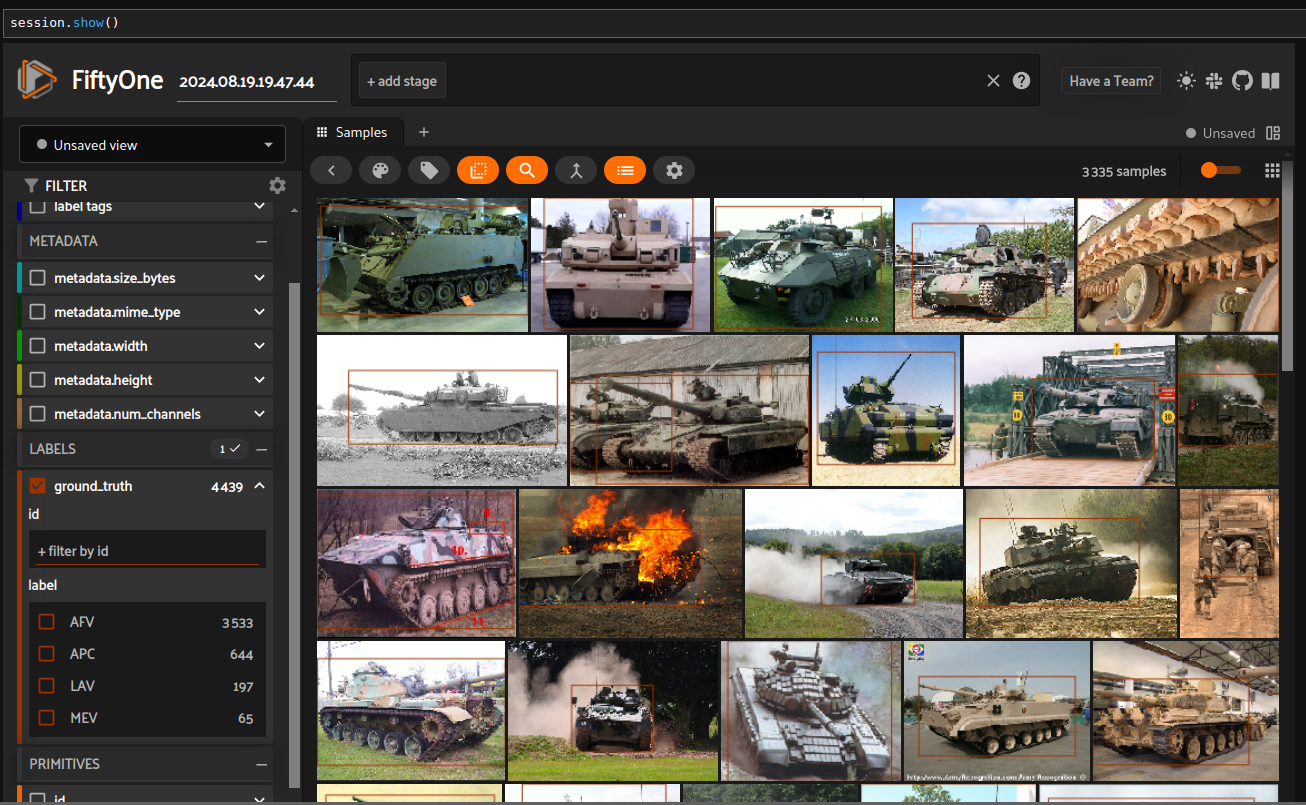
\includegraphics[width=\textwidth]{./images/fiftyone-dataset.png}
	\caption[Fiftyone dataset]{FiftyOne - Dataset (3335 images)}\label{fig:fiftyone-dataset}
\end{figure}

\subsubsection{Entrainement du modèle}

Pour la détection de véhicules militaires, en utilisant les datasets d'images annotées exportés, nous allons utiliser le model de base \textbf{YoloV8}.

De base, nous utilisons le modèle \textbf{yolov8m.pt} (medium), qui offre un bon compromis entre taille et vitesse, mais d'autres modèles que nous utiliserons pour l'expérience, sont disponibles auprès \textit{d'ultralytics}.

\begin{table}[h]
	\centering
	\begin{tabular}{|p{2cm}|p{2cm}|p{1.7cm}|p{2.4cm}|p{2.4cm}|p{1.7cm}|p{1.7cm}|}
		\hline
		\textbf{Model}   & \textbf{Size (pixels)} & \textbf{mAP\textsuperscript{val} 50-95} & \textbf{Speed CPU ONNX (ms)} & \textbf{Speed A100 TensorRT (ms)} & \textbf{Params (M)} & \textbf{FLOPs (B)} \\ \hline
		\textit{YOLOv8n} & 640                    & 37.3                                    & 80.4                         & 0.99                              & 3.2                 & 8.7                \\ \hline
		\textit{YOLOv8s} & 640                    & 44.9                                    & 128.4                        & 1.20                              & 11.2                & 28.6               \\ \hline
		\textit{YOLOv8m} & 640                    & 50.2                                    & 234.7                        & 1.83                              & 25.9                & 78.9               \\ \hline
		\textit{YOLOv8l} & 640                    & 52.9                                    & 375.2                        & 2.39                              & 43.7                & 165.2              \\ \hline
		\textit{YOLOv8x} & 640                    & 53.9                                    & 479.1                        & 3.53                              & 68.2                & 257.8              \\ \hline
	\end{tabular}
	\caption{Comparaison des modèles YOLOv8}
	\label{tab:yolov8_comparaison}
\end{table}

A ce niveau de l'expérience, la collecte des données du dataset d'entraînement c'est faite en deux grande étapes (Prepare-01 et Prepare-02).
Nous allons présenter les résultats d'entraînement avec et sans images non annotées avec des modèles de base de différences tailles.\\

La précision (\textbf{mAP : Mean Average Precision}) de notre modèle sera relevé à la fin de chaque entraînement afin de suivre son évolution.

\begin{equation}
	\text{mAP} = \frac{1}{N} \sum_{i=1}^{N} \text{AP}_i
\end{equation}

\begin{itemize}
	\item \textbf{N} : Représente le nombre total de classes dans le dataset.
	\item \textbf{AP$_i$} : Représente l'Average Precision (Précision Moyenne) pour la $i$-ème classe.
	\item \textbf{mAP} : Représente la moyenne des précisions moyennes sur toutes les classes.
\end{itemize}



\subsubsection*{Prepare-01: ImageNet, OpenImages, Roboflow (2666 images)}

A cette étape, le modèle détecte uniquement une classe 'tank', donc la mAP sera une moyenne de toutes les images.

J’ai essayé plusieurs scénarios sur l’algorithme en changeant le paramètres \textit{Epoch} (époques: passe complète à travers toutes les instances de dataset d'entraînement.) et la taille du modèles.


\begin{itemize}
	\item \textbf{yolov8m :}
	      \begin{itemize}
		      \item \textbf{Avec images non annotées :}
		            \begin{itemize}
			            \item Epoch = 60 $\Rightarrow$ mAP = 0.660601
			            \item Epoch = 80 $\Rightarrow$ mAP = 0.6548
			            \item Epoch = 100 $\Rightarrow$ mAP = 0.6476
		            \end{itemize}
		      \item \textbf{Sans images non annotées :}
		            \begin{itemize}
			            \item Epoch = 60 $\Rightarrow$ mAP = 0.71369
			            \item Epoch = 70 $\Rightarrow$ mAP = 0.692007695
			            \item Epoch = 80 $\Rightarrow$ mAP = 0.70
			            \item Epoch = 100 $\Rightarrow$ mAP = 0.70
		            \end{itemize}
	      \end{itemize}

	\item \textbf{yolov8l :}
	      \begin{itemize}
		      \item \textbf{Avec images non annotées :}
		            \begin{itemize}
			            \item Epoch = 60 $\Rightarrow$ mAP = 0.6512
			            \item Epoch = 80 $\Rightarrow$ mAP = 0.6491
			            \item Epoch = 100 $\Rightarrow$ mAP = 0.6384
		            \end{itemize}
	      \end{itemize}

	\item \textbf{yolov8x :}
	      \begin{itemize}
		      \item \textbf{Avec images non annotées :}
		            \begin{itemize}
			            \item Epoch = 60 $\Rightarrow$ mAP = 0.6518
			            \item Epoch = 80 $\Rightarrow$ mAP = 0.6535
			            \item Epoch = 100 $\Rightarrow$ mAP = 0.6308
		            \end{itemize}
	      \end{itemize}
\end{itemize}


Au vu de ces résultats, nous nous sommes rendu compte que la taille du modèle n'influence pas les résultats. Nous allons donc uniquement travailler avec la taille medium du modèle YoloV8.
Nous allons également utiliser des datasets contenant des images annotées.


\subsubsection*{Prepare-02: ImageNet, OpenImages, Roboflow and Google  (3335 images)}

A cette étape, nous avons entraîné le modèle a détecter les 04 classes (AFV, APC, MEV, LAV).
La moyenne mAP tient donc compte de ces 04 classes, mais nous allons aussi fournir la moyenne de chacune des classes.

\begin{itemize}
	\item \textbf{yolov8m :}
	      \begin{itemize}
		      \item Epoch = 60 $\Rightarrow$ mAP = 0.6609276140054803
	      \end{itemize}
\end{itemize}

\begin{figure}[h]
	\center
	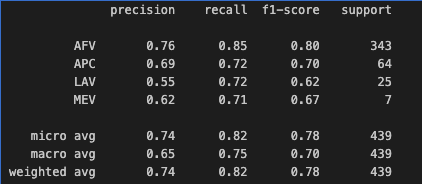
\includegraphics[width=0.6\textwidth]{./images/map-train.png}
	\caption[mAP des 04 classes]{mAP des 04 classes}\label{fig:map-train}
\end{figure}



\subsubsection{Suivi des objets}

Après avoir entraîné notre model avec notre jeu de donnée, nous utilisons le meilleur model (\textbf{best.pt}) obtenu pendant l'entraînement et un tracker (\textbf{bytetrack.yaml}) pour tracker les objets dans les vidéos.


\begin{figure}[h]
	\center
	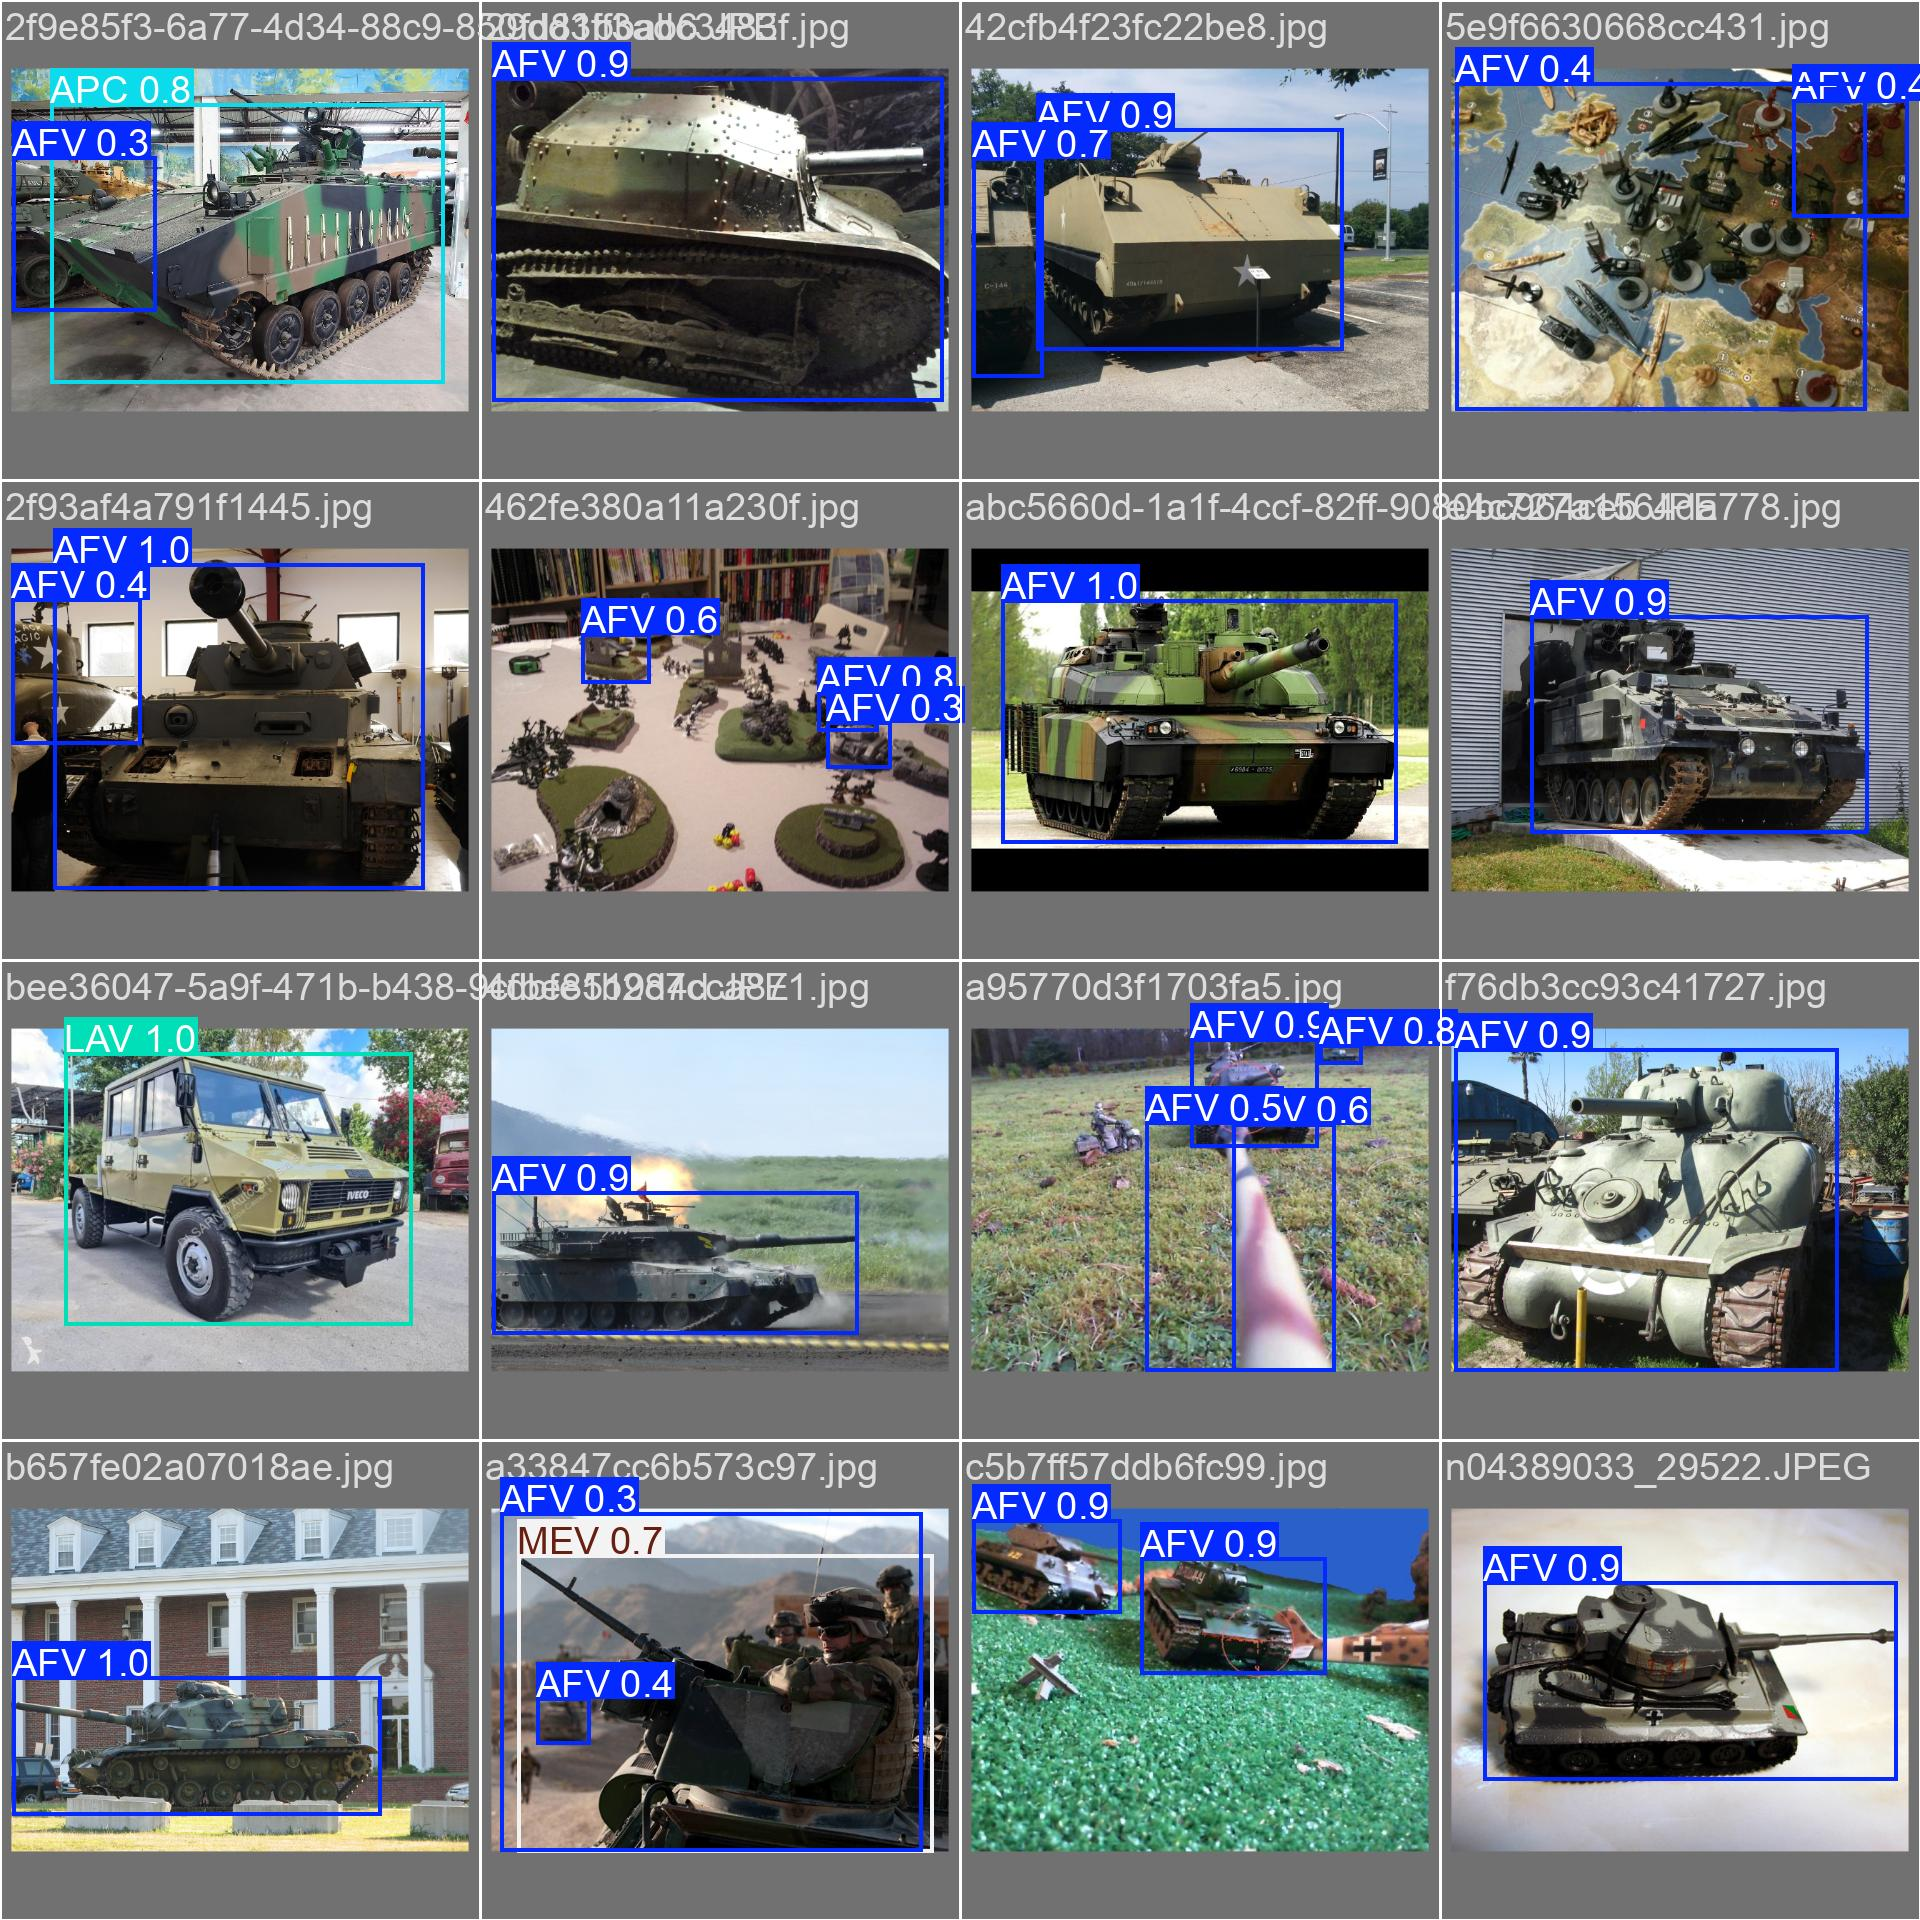
\includegraphics[width=0.8\textwidth]{./images/track2_val.jpg}
	\caption[Détection et reconnaissance avec taux de précision]{Détection et reconnaissance avec taux de précision}\label{fig:track2_val}
\end{figure}


\subsubsection{Génération d'images :}

Nous avons utilisé des méthodes d'augmentation des données afin d'améliorer la capacité du modèle à reconnaître des véhicules même lorsqu'ils sont éloignés ou partiellement masqués. Les méthodes utilisées incluent :

\begin{itemize}
	\item Une transformation \textbf{scale} pour dézoomer l'image et donner l'impression que le véhicule est vu de loin.
	\item Une transformation \textbf{XYMasking} pour masquer des bandes horizontales ou verticales, simulant un véhicule caché par un obstacle.
	\item Une transformation de type \textbf{Météo} pour donner l'impression qu'il y a de la neige, de la pluie ou du brouillard sur l'image.
\end{itemize}

\noindent Les étapes spécifiques suivies sont les suivantes :

\begin{enumerate}
	\item Dans un premier temps, nous avons récupéré une image de notre dataset avec ses labels (bounding boxes).
	\item Ensuite, nous avons créé une fonction qui applique les trois transformations à toutes les images du dataset.
	\item Enfin, nous avons entraîné le modèle YOLO avec ce dataset augmenté.
\end{enumerate}

Après l'augmentation des images, nous avons pu collecter en plus du dataset deja existant, \textbf{6670 images}.

Les résultats de l'entraînement seront dans l'annexe.

